\section{Outlook}

\setbeamertemplate{frame footer}{\cite{Patel2015}}
\begin{frame}
    \frametitle{Abdominal Aortic Aneurysm - Current Modelling Technique}
    \begin{columns}[onlytextwidth]
        \begin{column}{0.5\textwidth}
            \begin{itemize}
                \item Modelling from Aortic-Valve to Iliac-Bifurcation
                \item Modelling based on computer tomography (CT) or magnet resonance imaging (MRI)
                \item Rigid walls (only fluid domain modelled)
                \item Transient boundary conditions derived from literature
                \item Newtonian fluid model
                \item Transient simulation
                \item Simulation with commercial and open source CFD packages.
            \end{itemize}
        \end{column}
        \begin{column}{0.5\textwidth}
            \begin{figure}[ht]
                \centering
                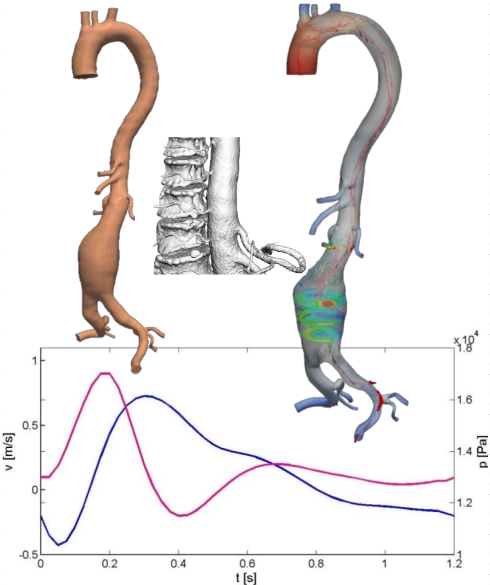
\includegraphics[width=0.7\textwidth]{aorta_current_modelling}
            \end{figure}
        \end{column}
    \end{columns}
\end{frame}
\begin{frame}
    \frametitle{Abdominal Aortic Aneurysm - Fluid Structure Interaction (FSI)}
    \begin{columns}[onlytextwidth]
        \begin{column}{0.5\textwidth}
            \begin{figure}[ht]
                \centering
                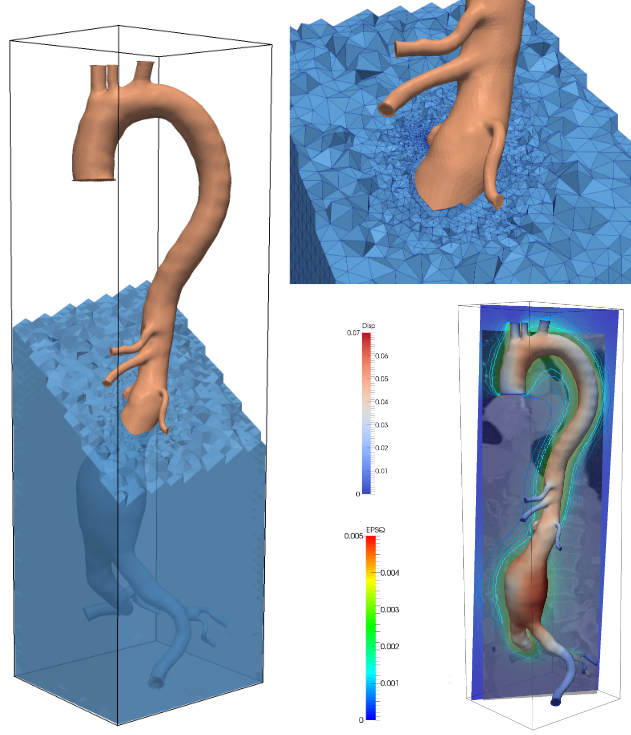
\includegraphics[width=0.7\textwidth]{aorta_fsi}
                \caption{Mesh-based approach - large scale problem}
            \end{figure}
        \end{column}
        \begin{column}{0.5\textwidth}
            \begin{figure}[ht]
                \centering
                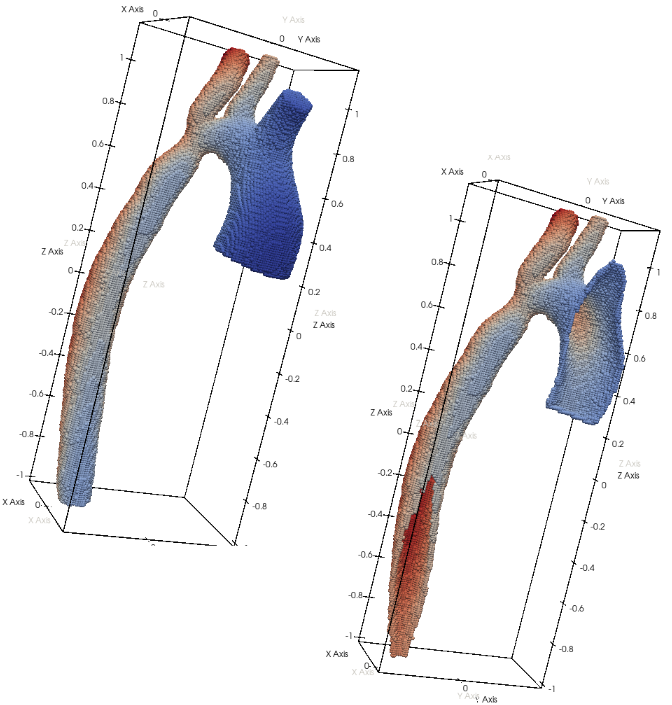
\includegraphics[width=0.8\textwidth]{aorta_particles}
                \caption{Particle-based approach - to be done ...}
            \end{figure}
        \end{column}
    \end{columns}
\end{frame}
